\documentclass[12pt, a4paper]{article}

\usepackage[hmargin=2.5cm, vmargin=2cm]{geometry}
\usepackage{amsthm, amssymb, mathtools, yhmath, graphicx}
\usepackage{fontspec, type1cm, titlesec, titling, fancyhdr, tabularx}
\usepackage{color, unicode-math, float, hhline}

\usepackage[CheckSingle, CJKmath]{xeCJK}
\usepackage{CJKulem}
\usepackage{enumitem}
\usepackage{tikz}
\usepackage{circuitikz}
%\setCJKmainfont[BoldFont=cwTex Q Hei]{cwTex Q Ming}
%\setCJKsansfont[BoldFont=cwTex Q Hei]{cwTex Q Ming}
%\setCJKmonofont[BoldFont=cwTex Q Hei]{cwTex Q Ming}
\setCJKmainfont[BoldFont=cwTeX Q Hei]{cwTeX Q Ming}

\def\normalsize{\fontsize{12}{18}\selectfont}
\def\large{\fontsize{14}{21}\selectfont}
\def\Large{\fontsize{16}{24}\selectfont}
\def\LARGE{\fontsize{18}{27}\selectfont}
\def\huge{\fontsize{20}{30}\selectfont}

%\titleformat{\section}{\bf\Large}{\arabic{section}}{24pt}{}
%\titleformat{\subsection}{\large}{\arabic{subsection}.}{12pt}{}
%\titlespacing*{\subsection}{0pt}{0pt}{1.5ex}

\parindent=24pt

\DeclarePairedDelimiter{\abs}{\lvert}{\rvert}
\DeclarePairedDelimiter{\norm}{\lVert}{\rVert}
\DeclarePairedDelimiter{\inpd}{\langle}{\rangle}
\DeclarePairedDelimiter{\ceil}{\lceil}{\rceil}
\DeclarePairedDelimiter{\floor}{\lfloor}{\rfloor}

\newcommand{\img}{\mathsf{i}}
\newcommand{\ex}{\mathsf{e}}
\newcommand{\dD}{\mathrm{d}}
\newcommand{\dI}{\,\mathrm{d}}

\setitemize{itemsep=0pt}
\setenumerate{itemsep=0pt}
\begin{document}

\section{四軸飛行器介紹}
\begin{figure}[H]
  \centering
  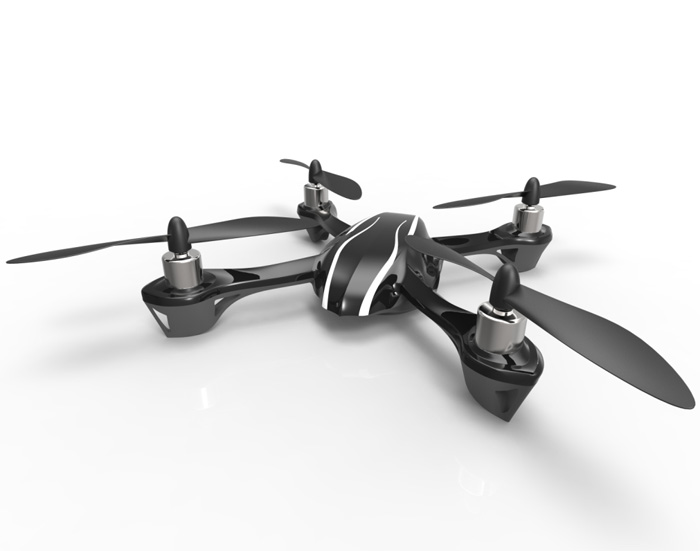
\includegraphics[width=0.4\textwidth]{Figures/quadcopter.jpg}
\caption{一個常見的四軸飛行器}
\label{fig:}
\end{figure}

\section{物理模型}
要維持四軸飛行器的平衡,須要考慮以下幾個物理量。
\begin{itemize}
  \item 外力造成的加速度,即 $a_x, a_y, a_z$ 。 
  \item 力矩造成的角加速度,即 $\alpha_x, \alpha_y, \alpha_z$ 。 
\end{itemize}
可以藉由控置馬達來條整四軸飛行器所受的力與力矩。
我們不妨假設四個馬達的推力分別為 $F_1, F_2, F_3, F_4$ 。

\subsection{升力}
四軸飛行器所受的升力即為四個馬達推力的總合,即
 \[ F = F_1 + F_2 + F_3 + F_4 \]

\subsection{力矩- $x, y$ 方向}
兩個對角的螺旋槳的升力差會使四軸飛行器受到一個 $x$ 或 $y$ 方向的力矩,
即
\[ \tau_x = (F_2 - F_4) r, \quad \tau_y = (F_3 - F_1) r \]
其中 $r$ 是 四軸的臂長(馬達到質心的距離)。

\subsection{力矩- $z$ 方向}
四軸飛行器的螺旋槳由1號到4號是正反轉交錯的,
而螺旋槳加速轉動時,或即使是等速轉動也會因
空氣的摩擦力,產生一個反方向的力矩。
 \[ \tau_z = F_1 - F_2 + F_3 - F_4 \]
 \begin{figure}[H]
  \centering
  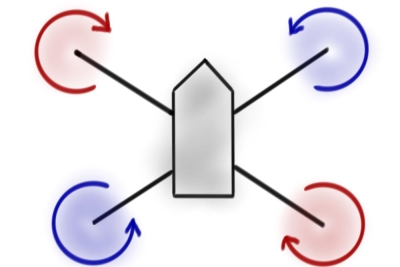
\includegraphics[width=0.4\textwidth]{Figures/prop-dir.jpg}
\caption{}
\label{fig:}
\end{figure}

\section{PID}
四軸飛行器是一個不隱定的系統,我們必須藉助電腦控置來達到平衡。
PID 控置就是一種方法。 首先我們設定一個目標態,比如若要四軸飛行器
平衡,目標應該設為
\[ z = 0, \; \theta_x = \theta_y = \theta_z = 0 \]
對於上例的每一項,我們都有對應的控制方法。
比如若要 $z$ 增加,我們應該提高升力,即各個馬達的轉速。
而若要 $\theta_x$ 減少,我們便應該提高4號馬達的轉速,
降低2號馬達的轉速。 我們把這種調整稱作對應的反應(action)。
假設 $x$ 是目標的值, 而 $x'$ 是實際的值, 即誤差為
$e = x - x'$ 。 現在我們必須跟據誤差來調整反應
$y$ 的大小。

PID 就利用比例項(P), 積分項(I) 以及微分項 (D) 來調控反應。
公式為
\[ y(t) = K_p e(t) + K_i \int_{0}^{t} e(\tau) \dI \tau + K_d \frac{\dD e(t)}{\dD t}\]
其中 $K_p, K_i, K_d$ 分別為 比例項(P), 積分項(I) 以及微分項 (D) 的增益。
\subsection{比例項(P)}
比例項顧名思義,就是和誤差正比的那一項, 即 $K_p e(t)$ 。
$K_p$ 太低會使得系統反應太慢, 太高會使得系統不穩定。
\subsection{積分項(I)}
積分項可以消除系統的偏差,如馬達實際轉速不同等等。
$K_i$ 太大也會使得系統不穩定。
\subsection{微分項(D)}
微分項可以有效的使系統穩定,但容易受感應器的誤差所影響。

\section{實作細節}
\subsection{PID}
你必須實作 \texttt{controller/pid.py} 中的 \texttt{class PID} 。 
其中必須包含函數 \\
\texttt{get\_control(self, t, err)} \\
輸入:
\begin{itemize}
  \item \texttt{t}: 當前的時間。
  \item \texttt{err}: 當前的誤差。
\end{itemize}
輸出: \\
一個浮點數 \texttt{y} 表示反應的大小。

\subsection{模擬器使用方法}
\texttt{python3 main.py -m sim} 來執行模擬器。
 
%\section{

\end{document}

